\documentclass[aspectratio=169]{beamer}

%Style


%Packages
\usepackage[utf8]{inputenc}
\usepackage{color}
\usepackage{graphicx}
\usepackage{booktabs}
\usepackage{lmodern}
\usepackage{amsfonts,amsmath,amssymb,amsthm}
\usepackage{varwidth}
\usepackage{mathtools}
\usepackage{xcolor}
\usepackage{framed}
\definecolor{shadecolor}{RGB}{180,180,180}
\usepackage{pgfplots}
\usetikzlibrary{arrows.meta}
\usepgfplotslibrary{groupplots}
\pgfplotsset{compat=newest}
\usetheme{HM}


%Title and Footer----------------------------------
\title[Enhanced PDR for Firefighting]{Enhanced Pedestrian Dead Reckoning Sensor Fusion for Firefighting}
\author{Tobias Augustin, Daniel Ossmann}
\institute[]{University of Applied Science Munich, HM}
\date{\today}
%--------------------------------------------------

\definecolor{HMRed}{RGB}{252 085 085}
\definecolor{HMRed2}{RGB}{254 184 184}
\definecolor{MYgray}{RGB}{140 136 136}
\definecolor{FK03}{RGB}{000,141,208}
\definecolor{lightgrey}{RGB}{207 200 200}
\definecolor{lightergrey}{RGB}{209, 207, 207}
\definecolor{green}{RGB}{013 189 016}
\definecolor{orange}{RGB}{235, 152, 052}
\definecolor{lila}{RGB}{162, 052, 235}

\definecolor{color2}{RGB}{65, 64, 112}

\definecolor{black}{RGB}{000 000 000}

\usetikzlibrary{positioning,plotmarks, matrix, arrows, calc, shapes}
\tikzstyle{blockdiag}	= [node distance=0mm, >=stealth', semithick]

%Hier beginnt die Präsentation
\begin{document}	
	% Title page frame
	{
	{\setbeamertemplate{footline}{}
	
		\begin{frame}
			\titlepage
		\end{frame}}
	\usebackgroundtemplate{ }
	
	\begin{frame}{Introduction}
		How miscommunication almost burned down a house:
		\begin{columns}
			\column{0.5\textwidth}
			\begin{figure}
				\centering
				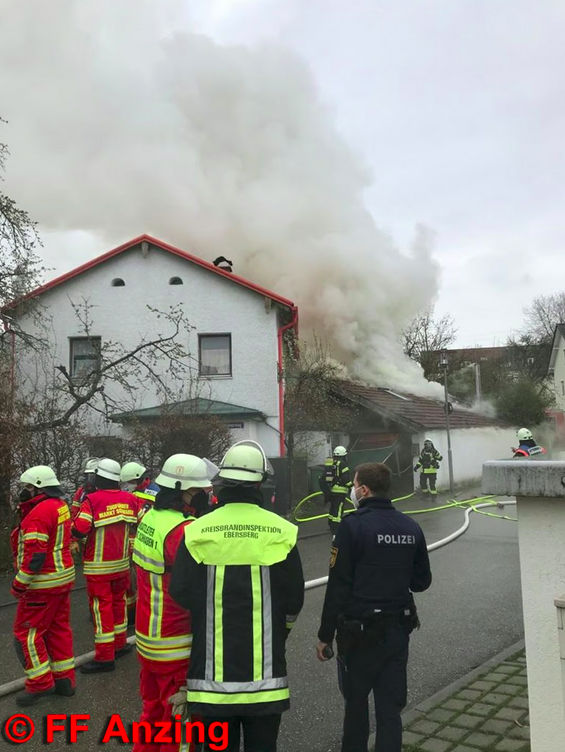
\includegraphics[height=0.7\textheight]{fire.png}
			\end{figure}
			
			\column{0.4\textwidth}
			\begin{figure}
				\centering
				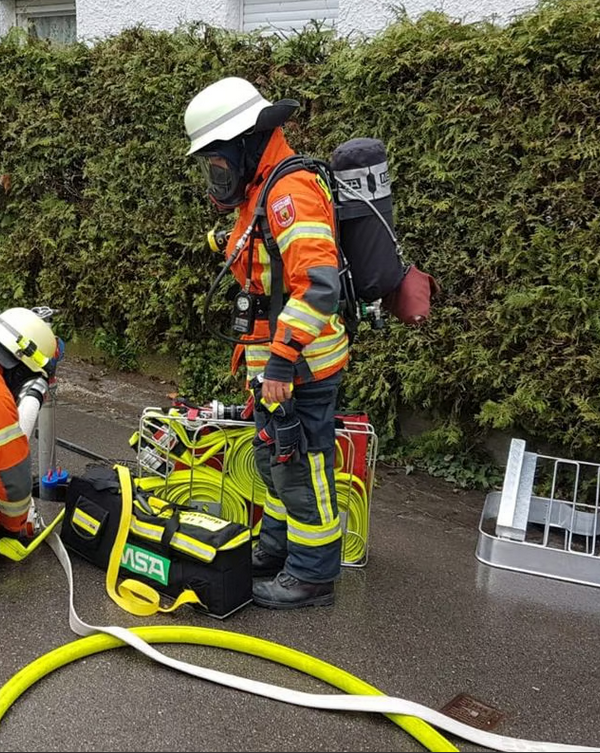
\includegraphics[height=0.7\textheight]{firefighter.png}
			\end{figure}
			
		\end{columns}
		
		
	\end{frame}
	
	\begin{frame}{Introduction}
			\begin{columns}
			\column{0.5\textwidth}
				\begin{itemize}
					\item<2-> Communication between leadership on the outside and firefighters in the building can be difficult and lead to further damages
					\item<3-> Knowing the position of injured firefighters could shorten rescue times
					\item<4-> Position tracking of firefighters can improve training effectiveness
					\item[$\blacktriangleright$]<5-> Requires a body worn system to track a firefighters position
				\end{itemize}
		
			\column{0.4\textwidth}
				\begin{figure}
					\centering
					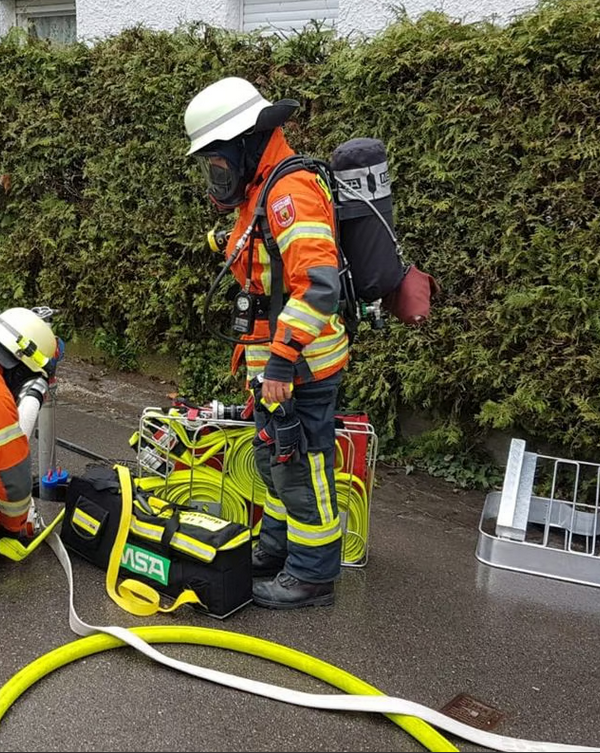
\includegraphics[width=0.7\textwidth]{firefighter.png}
				\end{figure}
	
		\end{columns}
		
		
	\end{frame}
	
	\begin{frame}{Requirements for Firefighting}
		\begin{itemize}
			\item Should not require prior setup of electronics
			\item Should be able to work in environments with smoke and high temperatures
			\item Lightweight and easy to carry % Should not impact movement
			\item Wireless data transmission possible % For leadership outside
			\item Low cost % Widespread use
		\end{itemize}
		
		\begin{block}{Problem:}
			$\blacktriangleright$ Existing solutions for indoor tracking can not meet these demands
		\end{block}
		
	\end{frame}
	
	\begin{frame}{Existing Solutions}
		\begin{itemize}
			\item Magnetic Triangulation $\rightarrow$ Requires expensive setup, not feasible for small departments 
			\item Lidar Sensors $\rightarrow$ Accuracy strongly influenced by smoke particles
			\item RF Localization 
			\item RF or magnetic field mapping $\rightarrow$ require prior setup
			\item Inertial measurement unit $\rightarrow$ prone to drift, needs secondary sensor
			\item Step detection $\rightarrow$ Accuracy affected by non walking movements
			\item[$\blacktriangleright$] What about an optical sensor?
		\end{itemize}
	\end{frame}
	
	
	\begin{frame}{Tracking Camera}
		\begin{itemize}
			\item Stereo-camera
			\item Calculates 3D information by measuring the horizontal difference of corresponding image points
			\item Intel RealSense T265 is used
			\item Works in environments with light smoke or bad lighting
		\end{itemize}
		
		
		\begin{figure}
			\centering
			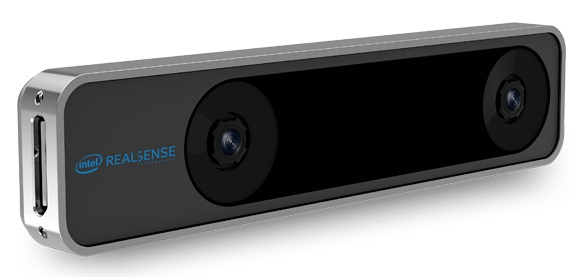
\includegraphics[width=0.45\textwidth]{realsense.jpg}
		\end{figure}
		
			\begin{block}{What if the optical sensor is obstructed by debris or heavy smoke?}
		\end{block}
	\end{frame}
	
	\begin{frame}{Step-Detection}
		\begin{itemize}
			\item Zero-crossing detection 
			\item Step-length estimation with $d = \sqrt[4]{a_{\max}-a_{\min}}  \, c$
			\item Step-length is added in the direction the individual is looking
		\end{itemize}
		
		\vspace{0.5cm}
		\begin{figure}
			\centering
			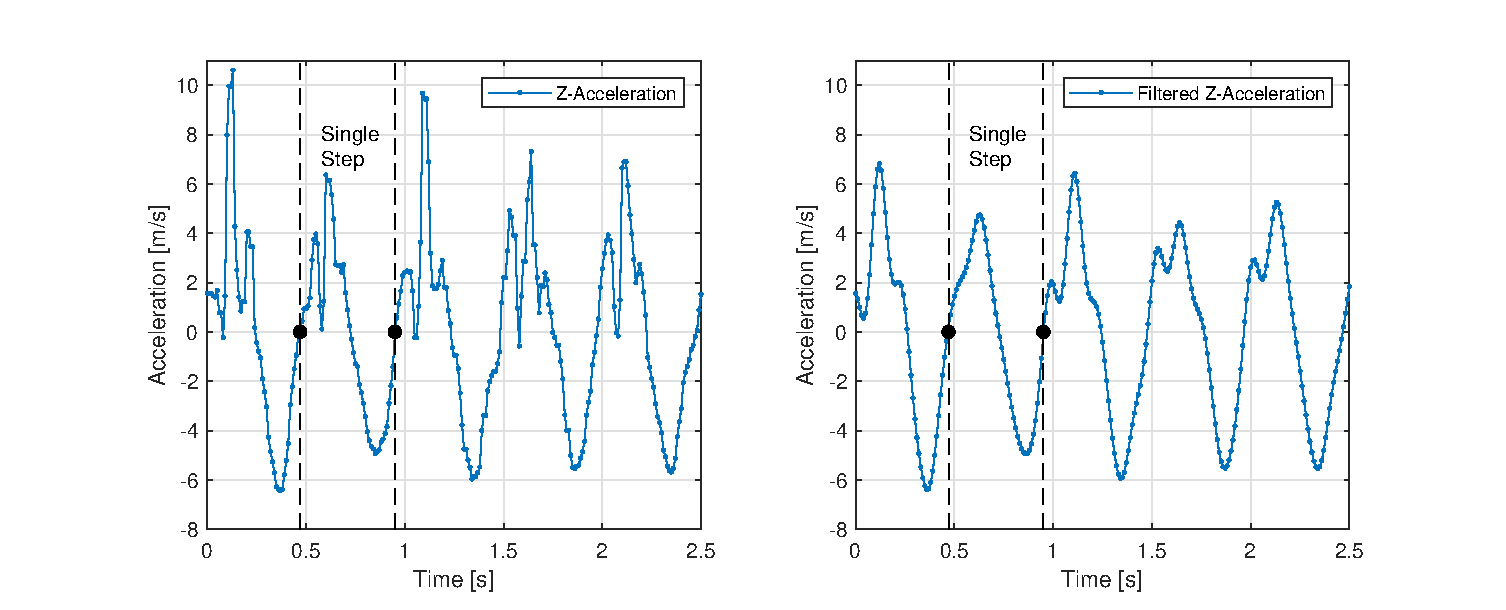
\includegraphics[width=0.9\linewidth]{../Conference_Paper/WalkAcceleration}
		\end{figure}
		
		
		
	\end{frame}
	
	\begin{frame}{Sensor-Data Fusion}
		\begin{itemize}
			\item Kalman filter for sensor-data fusion
			\item Prediction step assumes a constant acceleration between filter updates 
			\item Sensor estimates are used in the update step of the Kalman filter
		\end{itemize}
	\end{frame}
	
	\begin{frame}{Lab-Testing the System}
		\begin{itemize}
			\item Only lab-tests as a proof of concept and to tune the system
			\item Walked or moved in a crouching movement on a set trajectory
			\item Analysis of the deviation on defined checkpoints
			\item Sensor assembly mounted on the backplate of a breathing apparatus
		\end{itemize}
		\begin{figure}
			\centering
			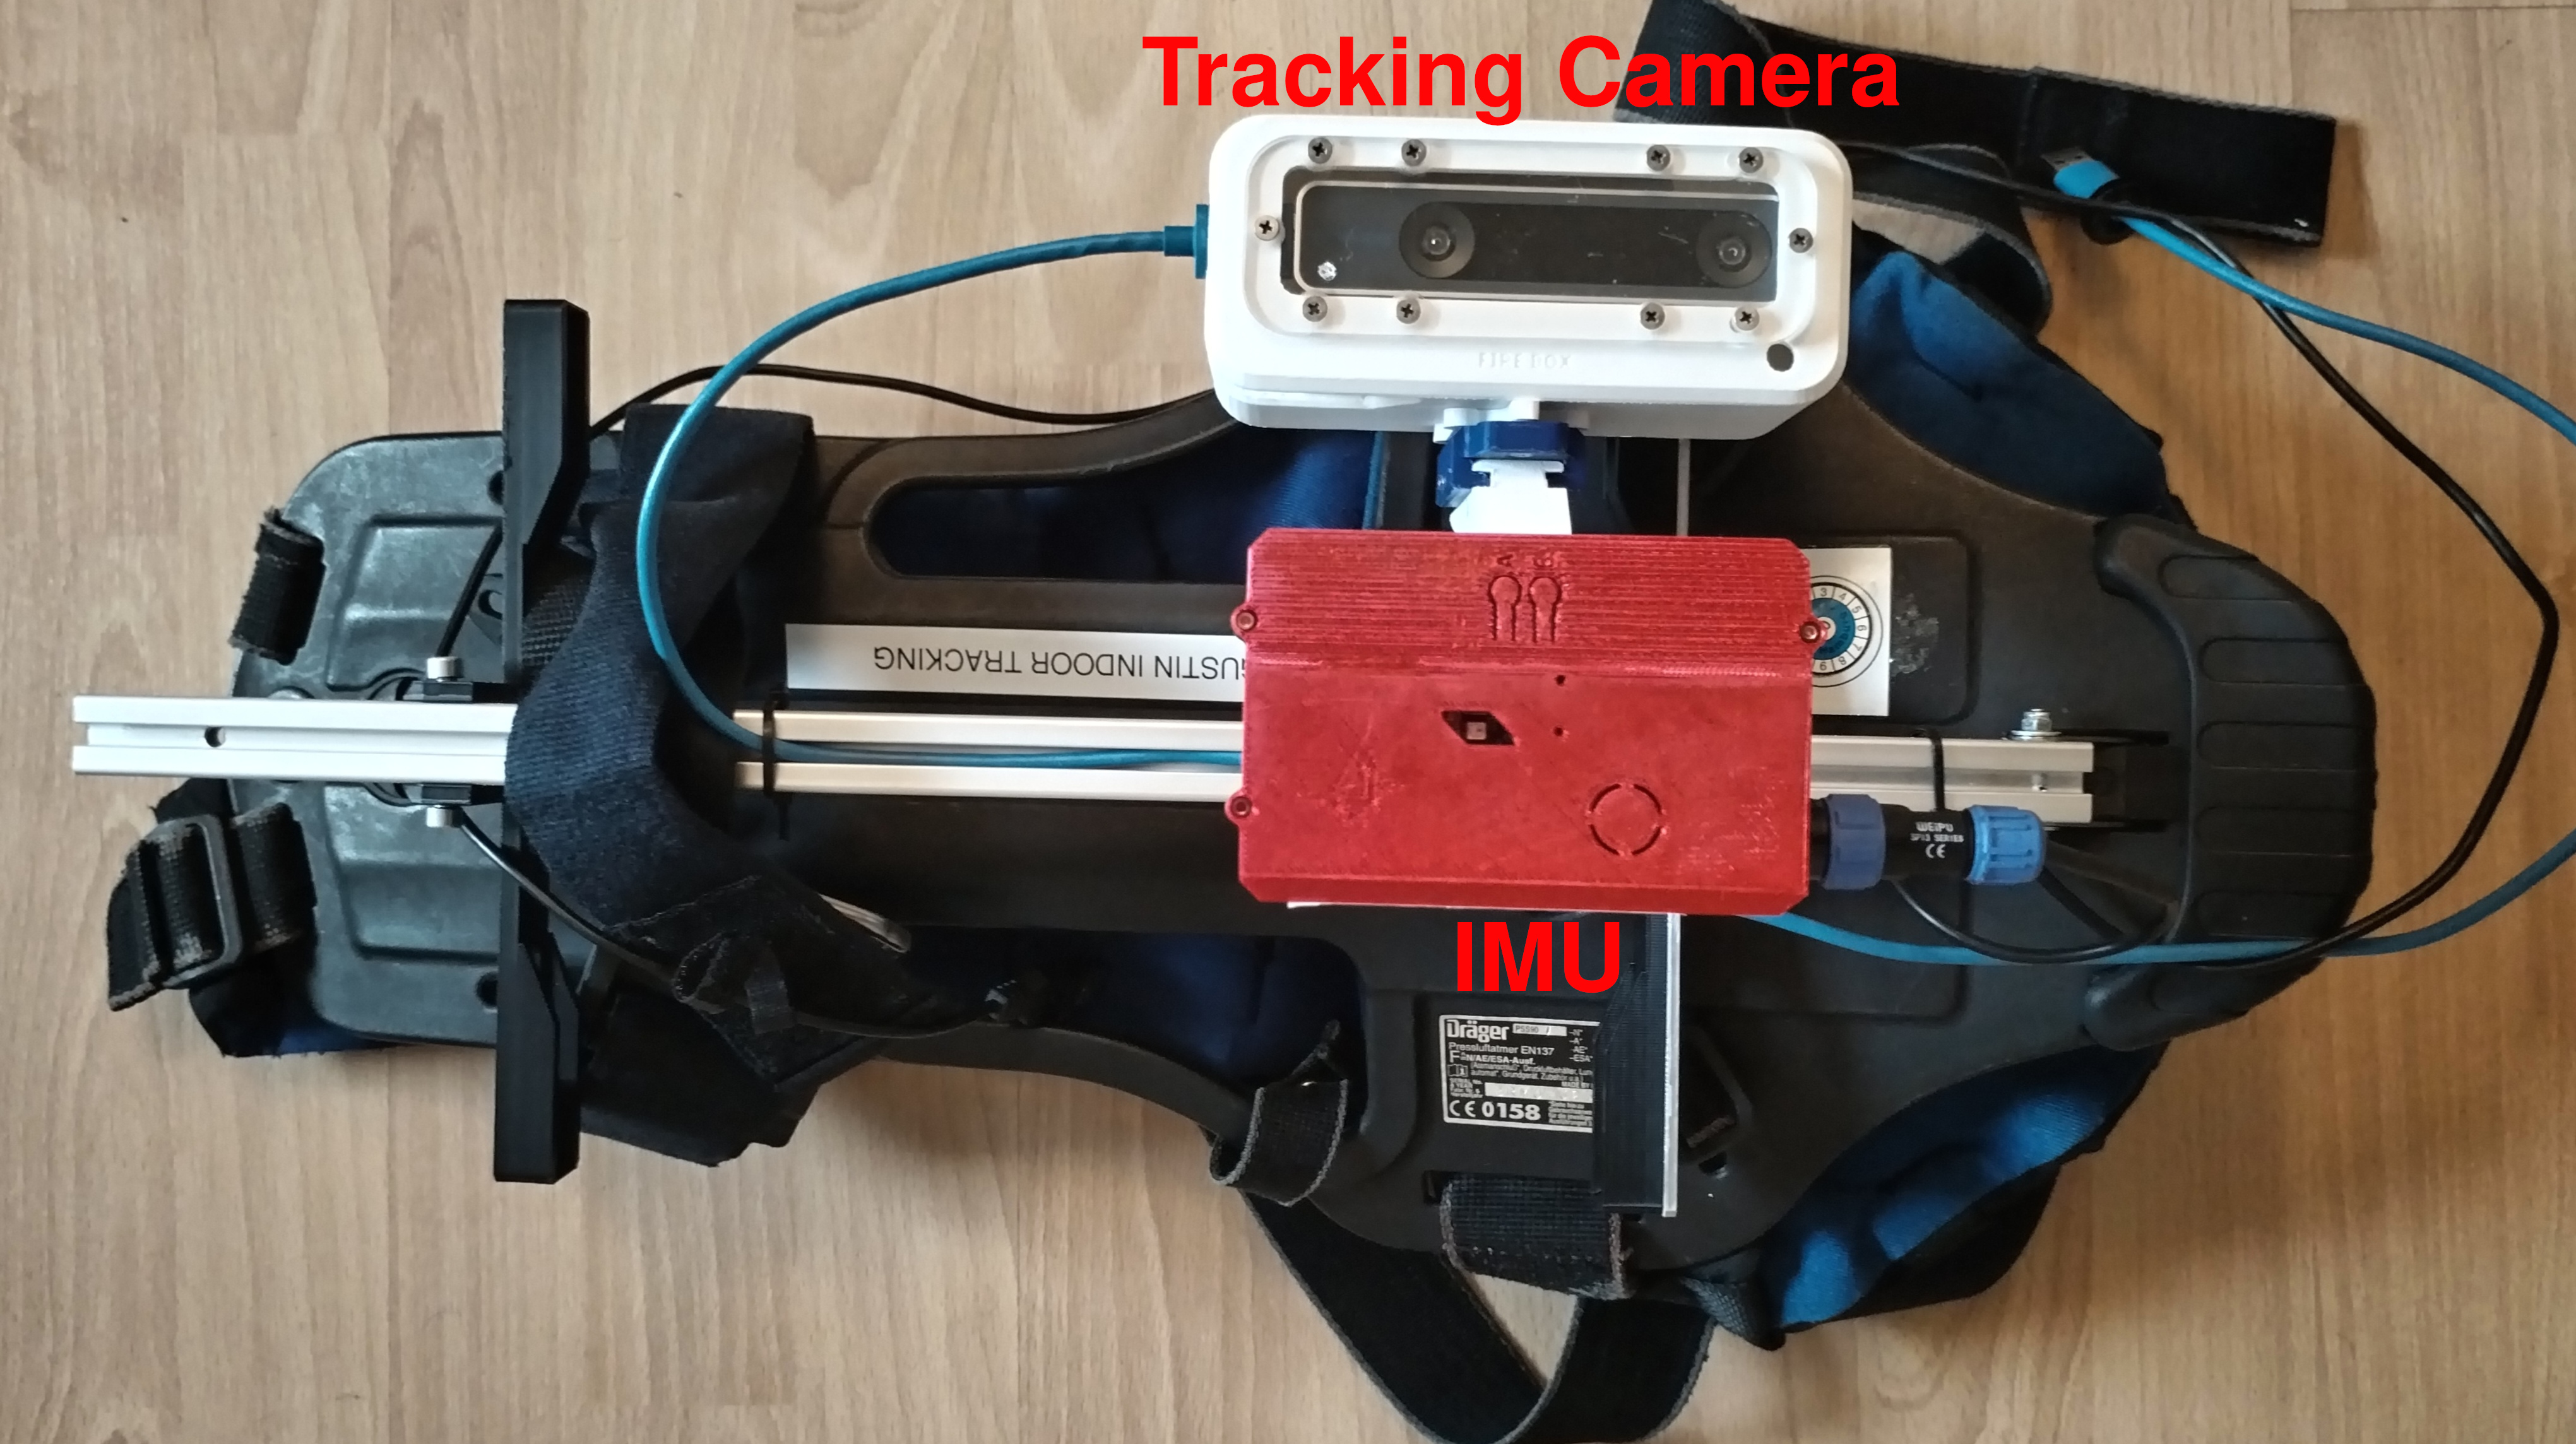
\includegraphics[width=7cm]{../Conference_Paper/Assembly.jpg}
		\end{figure}
		
	\end{frame}
	
	\begin{frame}{Results}
		\begin{columns}
			\begin{column}{0.45\textwidth}
				\begin{itemize}
					\item Significant improvement when the camera is used
					\item Accuracy when using only the tracking camera is slightly higher (in a lab environment)
					\item Step-detection accuracy goes down especially when crouching
				\end{itemize}
				
			\end{column}
			\begin{column}{0.54\textwidth}
				\begin{figure}
					\centering
					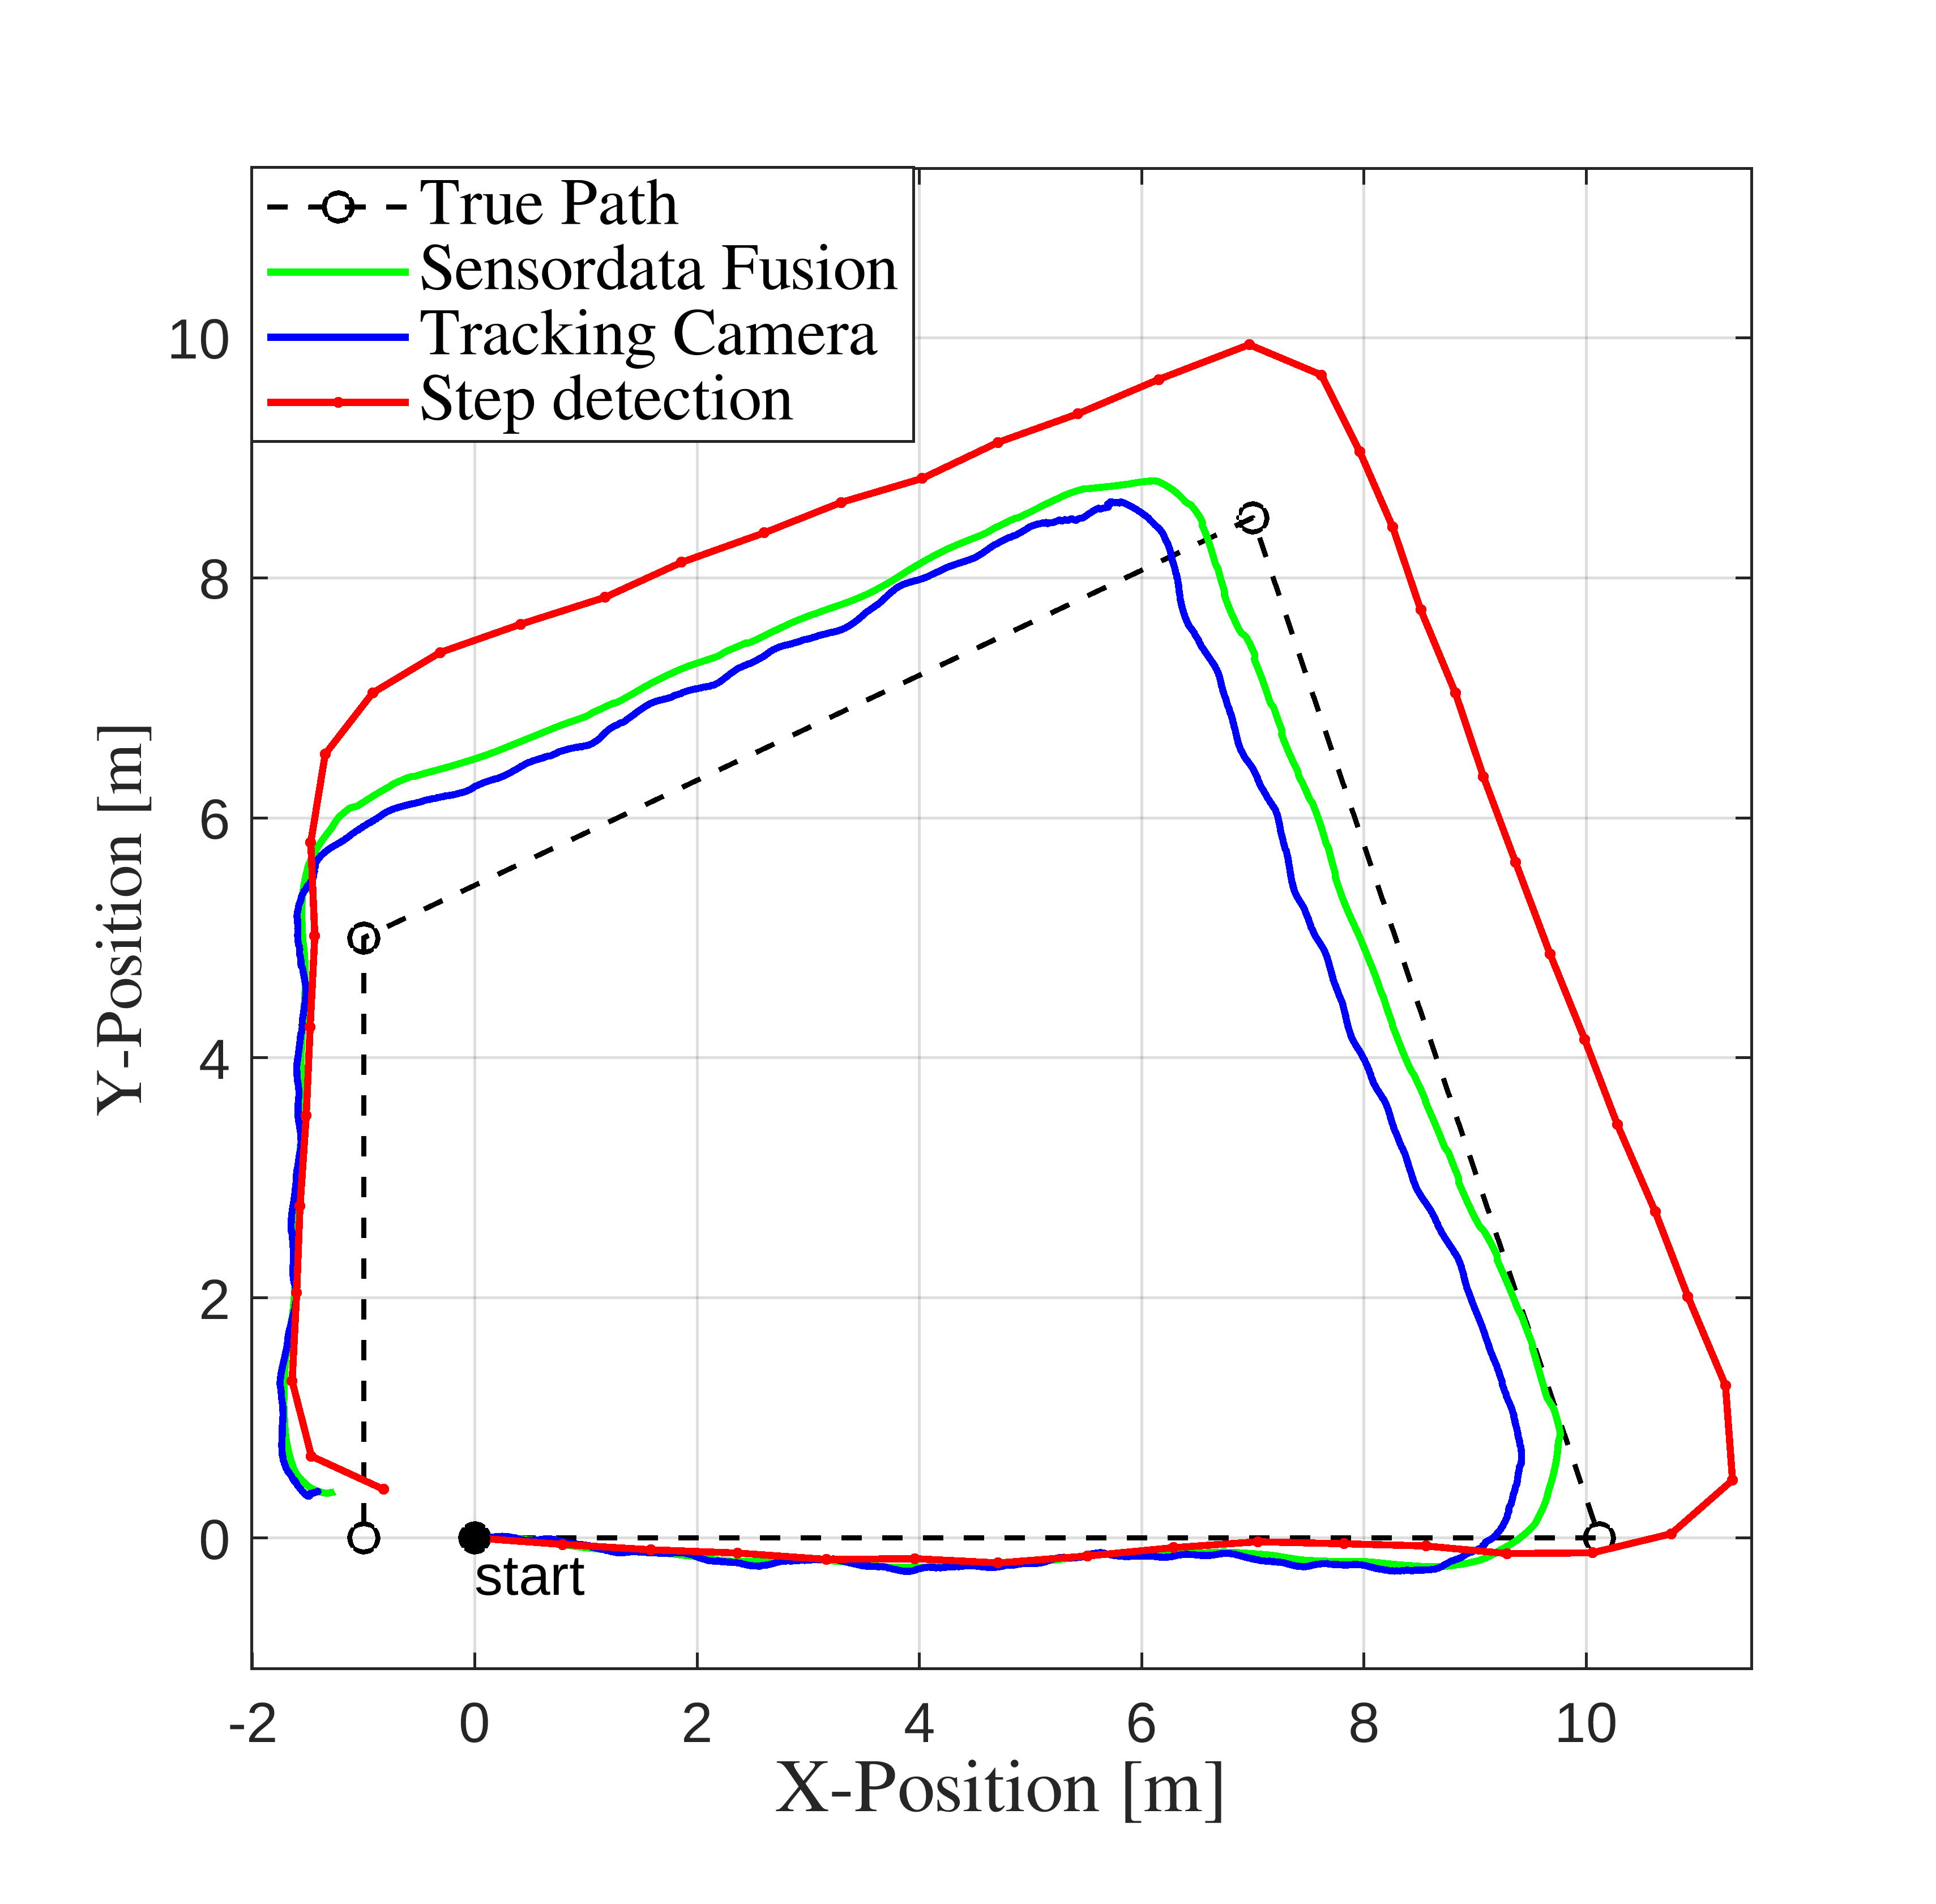
\includegraphics[width=0.9\linewidth]{../Conference_Paper/Path2}
					\caption{}
					\label{fig:path}
				\end{figure}
			\end{column}
					
			
		\end{columns}
	\end{frame}
	
	\begin{frame}{Conclusion}
		\begin{columns}
			\column{0.5\textwidth}
				\begin{itemize}
					\item While the results are promising, further research is necessary 
					\item Further tests in a firefighting environment are necessary (for example in a training container)
					\item[$\blacktriangleright$] Sensor assembly needs to be adapted for this task
				\end{itemize}
			\column{0.5\textwidth}
				\begin{figure}
					\centering
					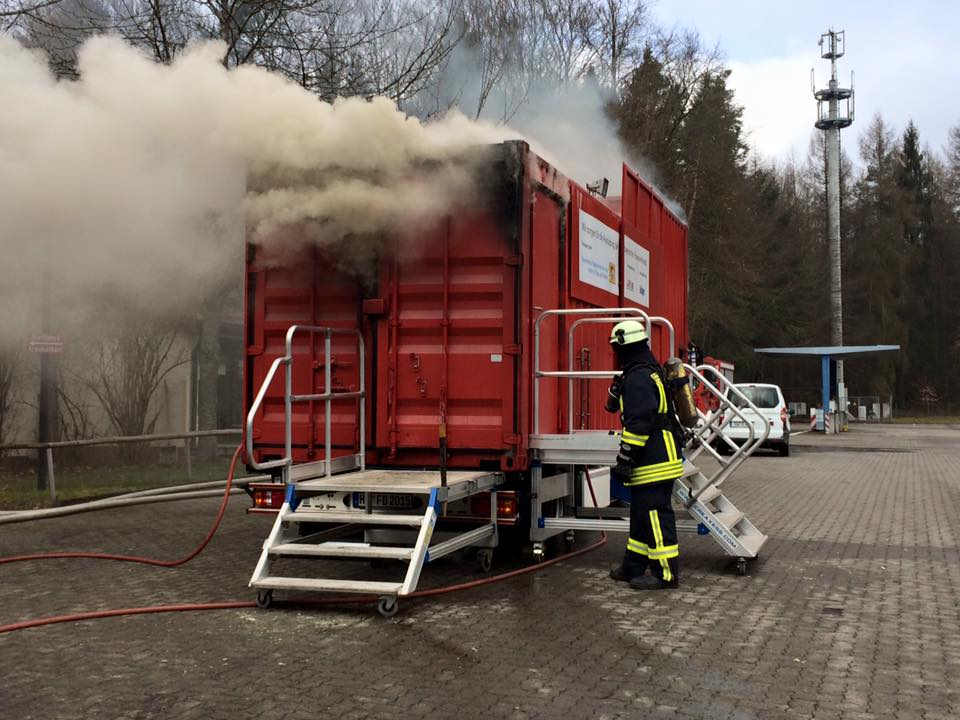
\includegraphics[width=0.8\textwidth]{Brandcontainer.jpg}
					%https://ffw-badbocklet.de/atemschutzgeraetetraeger-ueben-im-feststoff-brandcontainer/
				\end{figure}
			
		\end{columns}
		
		
	\end{frame}

	
\end{document}